\documentclass[10pt,a4paper]{article}

\usepackage[utf8]{inputenc}
\usepackage[T1]{fontenc}
\usepackage[margin=19mm]{geometry}
\usepackage{graphicx}
\usepackage{booktabs}
\usepackage{tabularx}
\usepackage{caption}
\usepackage{enumitem}
\usepackage{siunitx}
\usepackage{microtype}
\usepackage{titlesec}
\usepackage{xcolor}
\usepackage{hyperref}
\hypersetup{colorlinks=true,linkcolor=black,urlcolor=blue!50!black,citecolor=black}

\graphicspath{{figures/}}
\setlist{nosep,leftmargin=*}
\captionsetup{font=small,labelfont=bf,skip=3pt}
\sisetup{detect-all}
\newcolumntype{L}{>{\raggedright\arraybackslash}X}
\titlespacing*{\section}{0pt}{9pt}{4pt}
\titlespacing*{\subsection}{0pt}{7pt}{3pt}
\setlength{\parskip}{3pt}
\setlength{\parindent}{0pt}

\title{\vspace{-14mm}\textbf{On-Device Human Activity Recognition on an ESP32\\with Post-Training Int8 Quantisation}\\[3pt]
\normalsize Course project for Developing the Artificial Intelligence of Things (2026--2027), University of Helsinki}
\author{\normalsize Aakash Kangasasbai}
\date{\normalsize September 2026}

\begin{document}
\maketitle
\vspace{-10mm}
\begin{center}\small
Source code, model artefact and Wokwi diagram: repository \texttt{aiot-esp32-har} \quad$\cdot$\quad
Wokwi project: \url{https://wokwi.com/projects/475499882644462593}
\end{center}

% =====================================================================
\section{Prototype}

\textbf{Objectives and problem.} Wearable devices that recognise what a person is doing (walking, climbing stairs, sitting, lying) are the sensing front-end of fall detection, rehabilitation logging and context-aware building control. The na\"ive design streams raw inertial data to the cloud. For a 6-axis IMU at \SI{50}{\hertz} that is a continuous \SI{4.8}{kbit/s} of personally identifiable motion data; the radio carrying it dominates the energy budget and the round trip adds seconds of response latency. The course's principle of \emph{data minimisation} (Chapter~1.6) says never to transmit raw identifiable data when it can be avoided. The prototype therefore keeps the intelligence on the device, with three objectives: (1)~a deliberately designed sensing pipeline with measurable guarantees; (2)~an AI model running on the microcontroller, evaluated on people it has never seen; (3)~one edge-optimisation technique, post-training quantisation, applied with its parameters recorded and its effect on the accuracy--latency--size trade-off measured on the target. The result is an ESP32 that samples an MPU6050 at \SI{50}{\hertz}, classifies each \SI{2.56}{\second} window into six activities with an int8 1D-CNN, shows the result on an OLED and publishes it over MQTT.

\textbf{Evaluation in the context of Chapter 1.6.} The chapter argues that requirements should be \emph{falsifiable design hypotheses} (operating condition, observable metric, pass/fail threshold) and that every hardware iteration is an experiment on them. Table~\ref{tab:hyp} states the four hypotheses that shaped this prototype; each is checked by a counter the firmware prints, none is assumed. Two further themes of the chapter guided the design: \emph{cyber-physical resilience} (missed real-time deadlines make a model useless regardless of its accuracy, so the sampler is isolated from everything that can block) and \emph{data integrity} (messages are self-describing JSON carrying units and the measured rate, and only the class label leaves the device). The chapter's ``ideal network fallacy'' appeared in my own logs: the first MQTT integration silently broke the sampler during a one-second TCP connect.

\begin{table}[h]\small\centering
\caption{Design hypotheses (Chapter 1.6 form) and outcomes.}
\label{tab:hyp}
\begin{tabularx}{\textwidth}{@{}c L L L L@{}}
\toprule
\# & Operating condition & Metric & Threshold & Outcome \\
\midrule
H1 & Inference, display and network all active & Measured sampling rate; missed deadlines; dropped windows & $50\pm0.5$\,Hz, 0, 0 & \textbf{Pass}: 50.0\,Hz, 0, 0 (after three revisions) \\
H2 & People not in the training data & Test accuracy on held-out subjects & $\geq 90\,\%$, both models & \textbf{Pass}: 90.9\,\% / 91.2\,\% \\
H3 & Quantised model on the ESP32 & Accuracy loss; tensor arena; both models resident & $\leq 1$\,pt; $\leq 16$\,KB; yes & \textbf{Pass}: $+0.24$\,pt; 7.6\,KB; yes \\
H4 & Quantised inference on the ESP32 & Processing latency & int8 faster than float32 & \textbf{Fails in simulation} (446 vs 111\,ms); see \S\ref{sec:ai} \\
\bottomrule
\end{tabularx}
\end{table}

\textbf{Development process.} \emph{Board:} ESP32 DevKit-C over Pico and Uno. The Uno's \SI{2}{KB} RAM cannot hold the \SI{3}{KB} sample window; the Pico would fit the int8 model, but the ESP32's \SI{520}{KB} SRAM lets both the float32 and int8 models stay resident for comparison on identical inputs, its second core separates real-time sampling from inference, its two I2C controllers separate sensor and display, and its Wi-Fi enables the communication add-on. Every one of these features is used. \emph{Data:} Wokwi's MPU6050 is slider-driven and cannot generate a gait, so the model is trained on the UCI HAR dataset~\cite{anguita2013}: 30 subjects, waist-mounted MPU-class IMU, \SI{50}{\hertz}, the same physical quantities the sensor delivers. \emph{Iterations and abandoned approaches:}
\begin{enumerate}
  \item \emph{MaxPooling abandoned.} Its GPU gradient has no deterministic kernel, breaking bit-exact reproducibility; replaced by average pooling, accuracy unchanged.
  \item \emph{TensorFlow 2.16 abandoned.} Its converter cannot convert Keras-3 \texttt{Conv1D}; pinned 2.17.1.
  \item \emph{Inference in \texttt{loop()} abandoned.} 64 missed samples per inference because the sampler was starved. Inference moved to a FreeRTOS task on core~0, sampler alone on core~1.
  \item \emph{Shared I2C bus abandoned.} The OLED refresh ($\approx$\SI{25}{ms}) still blocked sensor reads; display moved to the second I2C controller.
  \item \emph{Networking in \texttt{loop()} abandoned.} A one-second TCP connect caused 36 missed deadlines; networking moved to core~0. H1 passed only then.
  \item \emph{\texttt{-Os} $\rightarrow$ \texttt{-O2}.} Seven-fold lower simulated latency for \SI{14}{KB} more flash: a size/latency trade-off in miniature.
\end{enumerate}

% =====================================================================
\section{Sensing pipeline}

\subsection{Hardware, sensors and communications}

\textbf{Sensor and signals.} MPU6050, 6-axis MEMS, 16-bit, configured for $\pm$\SI{2}{g} and $\pm$\SI{250}{\degree/s} (the range of human locomotion) with the on-chip digital low-pass filter at \SI{21}{\hertz}. Captured signals: three axes of total acceleration in g (gravity + body acceleration, encoding posture) and three axes of angular rate in rad/s (encoding rotation during gait). The sensor's Z axis is mounted along the dataset's ``vertical when upright'' axis.

\textbf{Reading mode: polling with a deadline scheduler.} Of the three modes in Chapter~1.3, streaming is unnecessary (14 bytes every \SI{20}{ms} on a \SI{400}{kHz} bus) and event-based acquisition, though the most energy-efficient on hardware, is unavailable because Wokwi's MPU6050 has no INT pin and the device is not power-limited here. Polling is done with a phase-locked deadline (\texttt{next = next + 20\,000\,\textmu s}, never \texttt{now + 20\,000}), so jitter cannot accumulate into drift. This is the temporal-alignment problem the chapter warns about. The firmware counts deadlines missed by more than one period and reports the \emph{measured} rate every second: the brief notes that a sensor configured for \SI{100}{\hertz} rarely delivers \SI{100}{\hertz}, and the answer is to measure rather than assume (H1).

\textbf{Sampling frequency: \SI{50}{\hertz}, set by the signal, not by energy.} Locomotion energy lies below 15--\SI{20}{\hertz}; Nyquist requires $\geq$\SI{40}{\hertz}, and \SI{50}{\hertz} adds margin and matches the training data. The \SI{21}{\hertz} on-chip filter is the anti-aliasing filter for $f_s/2=\SI{25}{\hertz}$. This is the opposite regime from the environmental topic, where a slow signal lets the period be chosen by the energy budget through duty cycling.

\textbf{Windowing and pre-processing.} A $128\times6$ ring buffer (\SI{3}{KB}); a window of 128 samples = \SI{2.56}{s} covers at least two gait cycles; inference every 64 new samples (50\,\% overlap) gives a decision every \SI{1.28}{s} at half the compute of per-sample inference. Window length and hop equal the dataset's segmentation. The per-channel mean and standard deviation of the training subjects are compiled into the firmware and applied by one function to live and replayed windows alike. This gives train/deploy parity.

\textbf{Concurrency.} Sampler in \texttt{loop()} on core~1; inference, OLED and network in a FreeRTOS task on core~0; IMU on I2C controller~0, OLED on controller~1. A window that arrives while inference is running is dropped and counted rather than delaying sampling. Under full load the result is \SI{50.0}{\hertz}, 0 missed, 0 dropped.

\textbf{Communication: MQTT publish--subscribe.} Each classified window is published as a $\sim$150-byte JSON message (source, label, both models' predictions, confidences, latencies, measured rate) to a public broker on the topic \texttt{aiot/har/<chip-id>/} \texttt{activity} with QoS~0; a browser dashboard subscribes over WebSockets. Publish--subscribe suits a constrained device because it never waits for a consumer, needs no server socket, and consumers can be added without touching the firmware; QoS~0 suffices because a lost label is superseded \SI{1.28}{s} later. The label channel carries $\approx$\SI{6}{bit/s} of information against \SI{4.8}{kbit/s} for the raw stream. This is the quantitative argument for edge inference. Cost: the Wi-Fi/TCP stack adds \SI{472}{KB} of flash (518 $\rightarrow$ \SI{991}{KB}) and its blocking connect had to be kept off the sampler core.

\textbf{Energy budget (estimate, datasheet values).} MPU6050 $\approx$\SI{3.9}{mA}; ESP32 $\approx$30--\SI{50}{mA} active at \SI{240}{MHz}, $\geq$\SI{100}{mA} while transmitting. Inference duty cycle \SI{111}{ms}/\SI{1.28}{s} $\approx 9\,\%$; radio active a few ms per window. The decision that matters most is \emph{what} is transmitted: one label instead of \SI{1.5}{KB} of raw samples per window keeps radio on-time near zero. Next step: light-sleep core~0 between windows and interrupt-driven acquisition so the sampler core can sleep between samples. This is the duty-cycling strategy of Chapter~1.3 at \SI{20}{ms} granularity.

\subsection{On-device AI}\label{sec:ai}

\textbf{Model.} 1D-CNN: Conv1D(16,$k$=5) $\rightarrow$ AvgPool(4) $\rightarrow$ Conv1D(32,$k$=5) $\rightarrow$ AvgPool(4) $\rightarrow$ Conv1D(32,$k$=3) $\rightarrow$ global average pooling $\rightarrow$ Dense(32) $\rightarrow$ Dense(6, softmax); 7\,446 parameters, sized for the device first. A CNN learns its own filters over the time axis instead of hand-crafted features. Training: Adam, batch 64, early stopping on validation subjects, seed 42, deterministic GPU kernels; 31 epochs in \SI{11}{s}.

\textbf{Evaluation protocol: subject-grouped split.} Chapter~2.3 explains that random splits of continuous sensing data leak: overlapping windows of the same person fall on both sides and the model is rewarded for recognising the person. The 30 subjects were partitioned 17 train (6\,054 windows) / 4 validation (1\,298) / 9 test (2\,947), with an assertion that the sets are disjoint. Every accuracy below is for unseen people.

\textbf{Optimisation technique: post-training quantisation, actual settings.} Following the chapter's ``quantise first'' advice, full-integer PTQ with the TFLite converter: operator set \texttt{TFLITE\_BUILTINS\_INT8}; weights int8, symmetric, \textbf{per-channel}; activations int8, asymmetric, per-tensor; biases int32; input and output tensors int8 (no float ops remain); calibration on 500 seeded training windows; resulting input scale 0.10107, zero-point $-6$; output scale $1/256$, zero-point $-128$. PTQ rather than QAT because the accuracy loss turned out to be zero; mixed precision was likewise unnecessary.

\begin{table}[h]\small\centering
\caption{Float32 baseline versus int8 PTQ (generated by \texttt{training/07\_summary.py}).}
\label{tab:results}
\begin{tabular}{@{}lrrl@{}}
\toprule
metric & float32 (before) & int8 PTQ (after) & change \\
\midrule
test accuracy, 9 unseen subjects ($n=2\,947$) & 90.94\,\% & 91.18\,\% & $+0.24$\,pt \\
macro-F1 & 0.909 & 0.911 & $+0.002$ \\
float $\leftrightarrow$ int8 prediction agreement & -- & 99.05\,\% & \\
weight bytes & 29\,784 & 7\,446 & 4.0$\times$ smaller \\
\texttt{.tflite} in flash & 36\,460\,B & 18\,352\,B & 2.0$\times$ smaller \\
tensor arena (ESP32 RAM) & 19\,792\,B & 7\,556\,B & 2.6$\times$ smaller \\
on-device accuracy, 18 replayed windows & 94.4\,\% & 88.9\,\% & \\
host $\leftrightarrow$ device agreement & 100\,\% & 94.4\,\% & \\
latency, Wokwi ESP32, \SI{240}{MHz}, \texttt{-O2} & 110.6\,ms & 446.4\,ms & int8 slower \emph{in simulation} \\
\bottomrule
\end{tabular}
\end{table}

\begin{figure}[h]\centering
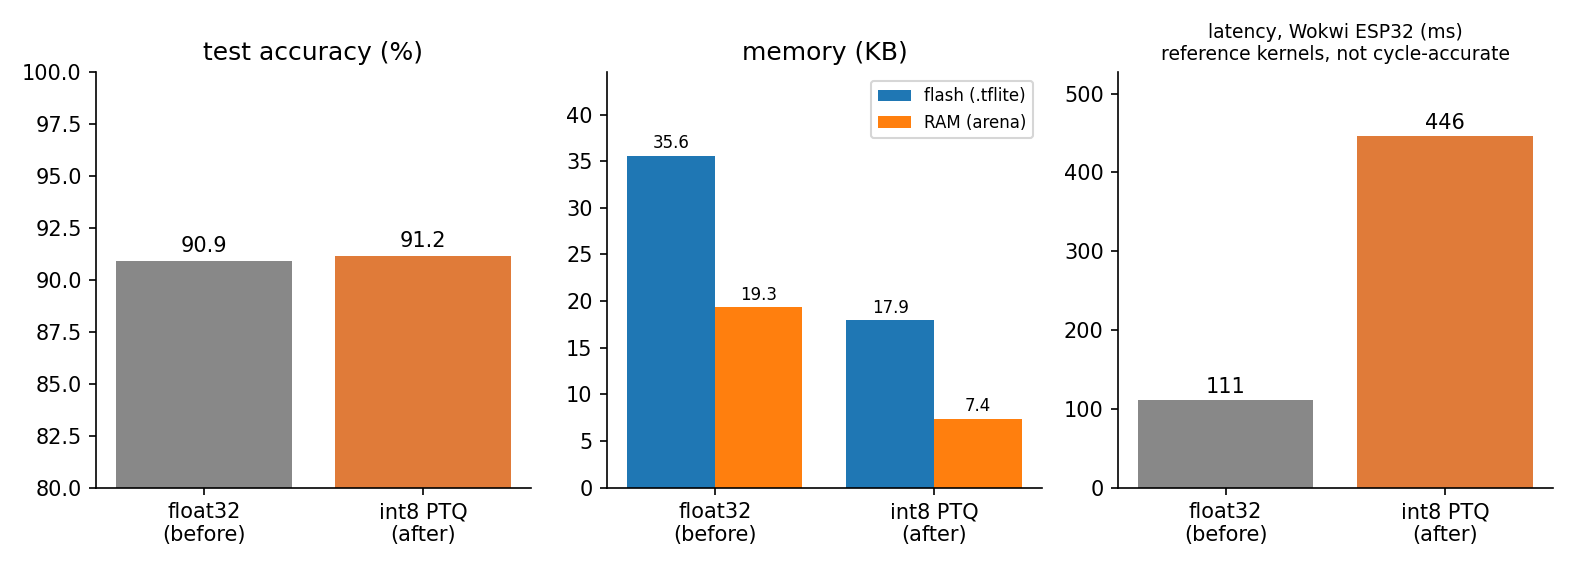
\includegraphics[width=\textwidth]{fig_tradeoff.png}
\caption{Before/after on the three axes of the edge-AI trade-off.}
\label{fig:tradeoff}
\end{figure}

\textbf{Accuracy.} Quantisation cost nothing: $+0.24$\,pt is within run-to-run noise and the models agree on 99\,\% of test windows. Both share one weakness: about a fifth of SITTING and STANDING windows are swapped. They are static postures with a near-identical gravity vector, so a \SI{2.56}{s} IMU window lacks the information to separate them. This is a limitation of the modality, not of the quantisation.

\textbf{Why PTQ was lossless: outlier weights and layer sensitivity.} Chapter~2.5 explains that quantisation degrades a model when a layer's range is stretched by outlier weights, crushing the resolution left for the many small informative weights, and that the damage compounds in early layers. Measured directly (Table~\ref{tab:weights}, Figure~\ref{fig:weights}): in every layer $\max|w|\leq 3.5\sigma$, the distributions are compact and approximately Gaussian, and per-channel scales give each output channel its own step of 0.003--0.0045. The most sensitive layer by this measure is the second convolution, which would be the first kept in higher precision had a loss appeared.

\begin{table}[h]\small\centering
\caption{Per-layer weight ranges of the float32 model.}
\label{tab:weights}
\begin{tabular}{@{}lrrrrr@{}}
\toprule
layer & weights & min & max & $\max|w|/\sigma$ & int8 step \\
\midrule
conv1d & 480 & $-0.507$ & 0.523 & 2.62 & 0.0040 \\
conv1d\_1 & 2\,560 & $-0.411$ & 0.337 & 3.33 & 0.0029 \\
conv1d\_2 & 3\,072 & $-0.477$ & 0.493 & 3.48 & 0.0038 \\
dense & 1\,024 & $-0.533$ & 0.561 & 2.79 & 0.0043 \\
dense\_1 & 192 & $-0.672$ & 0.470 & 2.57 & 0.0045 \\
\bottomrule
\end{tabular}
\end{table}

\begin{figure}[h]\centering
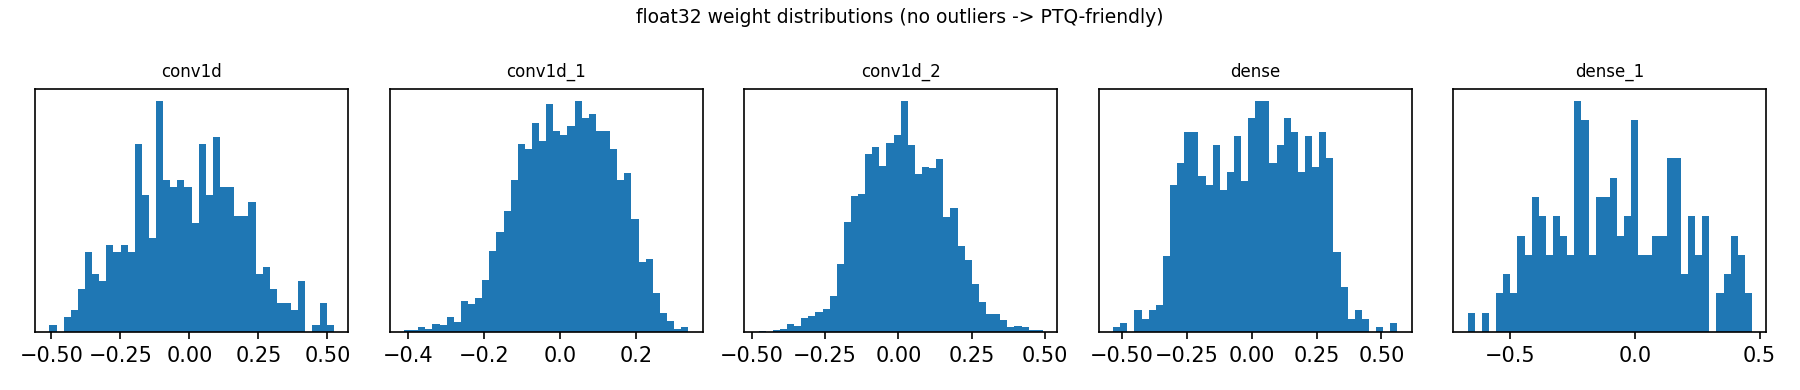
\includegraphics[width=0.95\textwidth]{fig_weights.png}
\caption{Float32 weight distributions per layer: compact, no outliers.}
\label{fig:weights}
\end{figure}

\textbf{Size.} Weights shrink exactly 4$\times$; the \texttt{.tflite} file only 2$\times$ because on a 7\,k-parameter model the flatbuffer structure and per-channel quantisation parameters are a large fixed overhead. The number that matters on the device is RAM: the tensor arena drops from \SI{19.8}{KB} to \SI{7.6}{KB} because int8 activations are a quarter the size of float32 ones.

\textbf{Latency: a negative result.} In Wokwi the int8 model is four times \emph{slower}. Three facts explain it: (i)~Wokwi is functionally accurate but not cycle-accurate. A micro-benchmark in the repository shows 170\,000 float multiply-accumulates take \SI{167}{ms} of simulated time ($\approx$240 simulated cycles each; real silicon needs 10--20) and 64-bit integer arithmetic is four times slower again; (ii)~the TensorFlow Lite Micro library used contains only \emph{reference} kernels, whose int8 requantisation uses 64-bit multiplies, which is exactly the operation the simulator penalises; (iii)~on a physical ESP32 with Espressif's ESP-NN kernels the int8 convolution is the accelerated path. The simulation measures an unoptimised software path, not the arithmetic. Enabling MQTT raised float latency from 87 to \SI{111}{ms} because core~0 also runs the network stack.

\textbf{Position on the Pareto frontier.} The course frames the accuracy--latency--size trilemma and the Pareto frontier as the set of configurations where improving one property costs another. On this device the int8 model \emph{dominates} float32 on two axes at equal accuracy (4$\times$ less weight memory, 2.6$\times$ less RAM, $+0.24$\,pt), so it is strictly closer to the frontier. On the third axis the outcome depends on the integer execution path beneath the model: for the simulated ESP32 with reference kernels the measured frontier is ``int8 for memory, float32 for latency''; for a physical ESP32 with optimised kernels int8 wins on all three. ``Moving toward the frontier for the chosen device'' is a statement about the device as much as about the model.

\textbf{Host versus device.} The same 18 held-out windows give identical float32 predictions on host and device and 17/18 identical int8 predictions; the one flip is a borderline STANDING window (device confidence 0.57, host 0.81), as TFLite and TFLite Micro round their requantisation differently. A quantised model must be validated on the target.

% =====================================================================
\section{Self-Reflection}

\textbf{Limitations and how to address them.} (a)~SITTING vs STANDING: inherent to a waist IMU over \SI{2.56}{s}; longer context, a barometer, or transition-aware event-based metrics (Chapter~2.3). (b)~Live dynamic classes cannot come from a slider-driven sensor; walking-type classes are demonstrated by injecting recorded windows from held-out subjects through the identical on-device path, labelled \texttt{INJECT}/\texttt{REPLAY}; a physical MPU6050 removes this. (c)~Latency is simulator-bound; a physical ESP32 with ESP-NN kernels would complete H4. (d)~Energy is estimated, not measured; sleep modes and interrupt-driven acquisition are the follow-ups. (e)~Labels go in clear to a public broker; TLS, a private broker and keys in a secure element are needed before deployment (Chapter~1.6). (f)~The axis mapping assumes the dataset's sensor placement; orientation calibration or rotation augmentation would make the model placement-robust.

\textbf{One course concept: grouped (leave-subjects-out) evaluation.} \emph{What it means:} in continuous sensing, consecutive windows from the same person, device or session are correlated through gait rhythm, sensor bias and posture habits. A random split scatters them across train and test, and the evaluation leaks: the model can score by recognising the source rather than the activity. Grouped evaluation conditions the split on the variable that causes the dependency, so every test window comes from an entity never seen in training; leave-one-subject-out is the strict form, a fixed held-out subject set the lighter one. \emph{Why it matters for AIoT:} evaluation must answer ``does it actually work?'' for devices deployed on people and environments absent from the lab; accuracy under a leaky protocol predicts nothing, accuracy under a grouped protocol estimates robustness. It also protects the optimisation study: an inflated baseline would make ``accuracy loss after quantisation'' meaningless. \emph{How I applied it:} 30 subjects split 17/4/9 into disjoint sets, asserted in code; early stopping on the validation subjects only; the 18 on-device replay windows drawn from the test subjects. \emph{What I observed:} training accuracy reached 97\,\% while unseen-subject accuracy settled at 91\,\% (Figure~\ref{fig:training}); that six-point gap is the real cost of generalising across people. It is exactly the gap a random split would have hidden, and it exposed SITTING/STANDING as a cross-subject problem rather than something a model could memorise away.

\begin{figure}[h]\centering
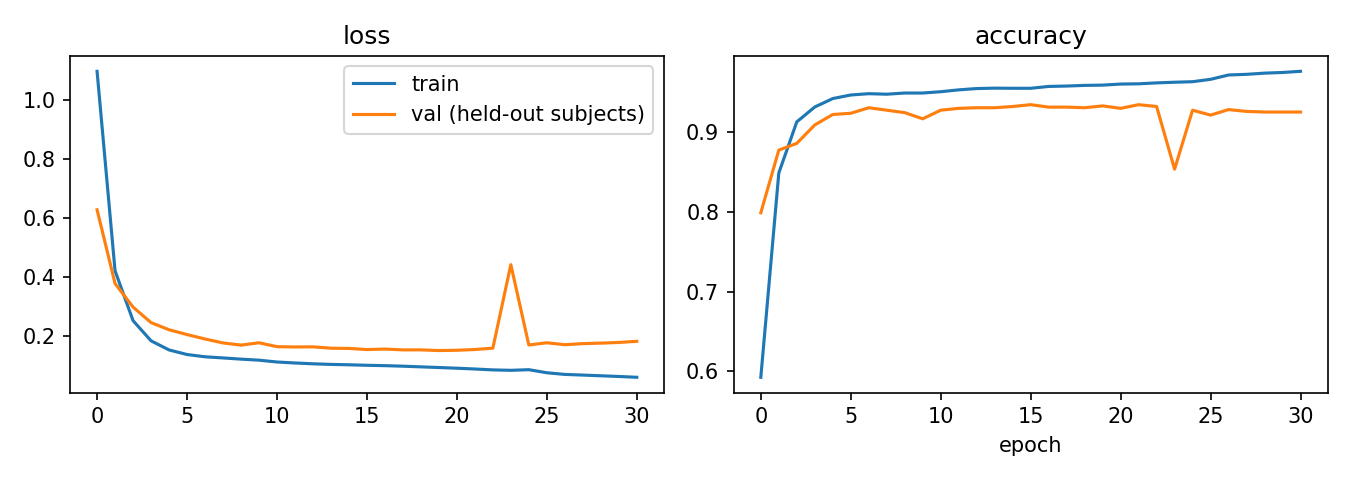
\includegraphics[width=0.8\textwidth]{fig_training.png}
\caption{Training curves; validation on four held-out subjects.}
\label{fig:training}
\end{figure}

\textbf{How my understanding of AIoT evolved.} I began thinking of an AIoT device as a small computer that runs a model and of this project as a compression exercise. Building it moved the centre of gravity to the system: the model took an afternoon, the sensing pipeline took three architectural revisions before it met something as basic as ``sample at \SI{50}{\hertz} while doing everything else''. Quantisation, which I expected to be the headline, was almost free on the accuracy axis and hardware-dependent on the latency axis; a technique cannot be judged apart from the device it runs on. The evaluation protocol decided what I could claim, and the communication design turned the energy and privacy case for edge AI into numbers. Chapter~1.6 changed my working method most: requirements as hypotheses with a counter behind each turned debugging into experiments, which is why the missed-deadline counter, not the confusion matrix, is the number I value most in this project.

% =====================================================================
\section*{Declaration of AI-tool use}
\textbf{AI tool used:} Claude Code (Anthropic). \textbf{Model/version:} Claude Opus 5 (\texttt{claude-opus-5}), September 2026. \textbf{Purpose:} grammar correction and formatting support (such as figure placement) for the final report; code debugging during development; and conceptual guidance for navigating the IoT toolchain, specifically assisting with the integration of the ESP32 firmware and Wokwi simulations.

\begin{thebibliography}{9}\small
\bibitem{anguita2013} D.~Anguita, A.~Ghio, L.~Oneto, X.~Parra, J.~L.~Reyes-Ortiz, ``A Public Domain Dataset for Human Activity Recognition Using Smartphones,'' \emph{ESANN}, 2013.
\bibitem{course} \emph{Developing the Artificial Intelligence of Things} (2026--2027), University of Helsinki MOOC: Chapters 1.3, 1.4, 1.6, 2.3, 2.5.
\end{thebibliography}
\end{document}
